\problemname{Soccer Stadium}

Nagyerdő is a square-shaped forest located in the city of Debrecen,
which can be modeled as an $N \times N$ grid of cells. The columns of
the grid are numbered from $0$ to $N - 1$ from west to east and the
rows are numbered from $0$ to $N - 1$ from north to south. We refer
to the cell located at row $r$ and column $c$ of the grid as cell
$(r, c)$.

In the forest, each cell is either \textbf{empty} or contains a
\textbf{tree}. At least one cell in the forest is empty.

DVSC, the famous sports club of the city, is planning to build a new
soccer stadium in the forest. A stadium of size $s$ (where
$s \ge 1$) is a set of $s$ \emph{distinct empty} cells
$(r_0, c_0), \ldots, (r_{s - 1}, c_{s - 1})$. That is, for each $i$
from $0$ to $s - 1$, inclusive, cell $(r_i, c_i)$ is empty, and
for each $j$ such that $i < j < s$, $r_i \neq r_j$ or
$c_i \neq c_j$ holds.

Soccer is played using a ball that is moved around the cells of the
stadium. A \textbf{straight kick} is defined to be either of the
following two actions:
\begin{itemize}
  \item Move the ball from cell $(r,a)$ to cell
  $(r,b)$ ($0 \le r,a,b < N, a \ne b$), where the stadium contains
  \emph{all} cells between cell $(r,a)$ and $(r,b)$ in row $r$.
  Formally,
  \begin{itemize}
    \item if $a < b$ then the stadium should contain cell
    $(r,k)$ for each $k$ such that $a \le k \le b$,
    \item if $a > b$
    then the stadium should contain cell $(r,k)$ for each $k$ such that
    $b \le k \le a$.
  \end{itemize}
  \item Move the ball from cell $(a,c)$ to cell $(b,c)$
  ($0 \le c,a,b < N, a \ne b$), where the stadium contains \emph{all}
  cells between cell $(a,c)$ and $(b,c)$ in column $c$. Formally,
  \begin{itemize}
    \item if $a < b$ then the stadium should contain cell $(k,c)$ for each
  $k$ such that $a \le k \le b$,
    \item if $a > b$ then the stadium
  should contain cell $(k,c)$ for each $k$ such that
  $b \le k \le a$.
  \end{itemize}
\end{itemize}


A stadium is \textbf{regular} if it is possible to move the ball from
any cell contained by the stadium to any other cell contained by the
stadium with at most $2$ straight kicks. Note that any stadium of size
$1$ is regular.

For example, consider a forest of size $N = 5$, with cells $(1,0)$
and $(4,2)$ containing trees and every other cell being empty. The
figure below shows three possible stadiums. Cells with trees are
darkened, and cells contained by the stadium are striped.

\begin{figure}[h!]
\centering
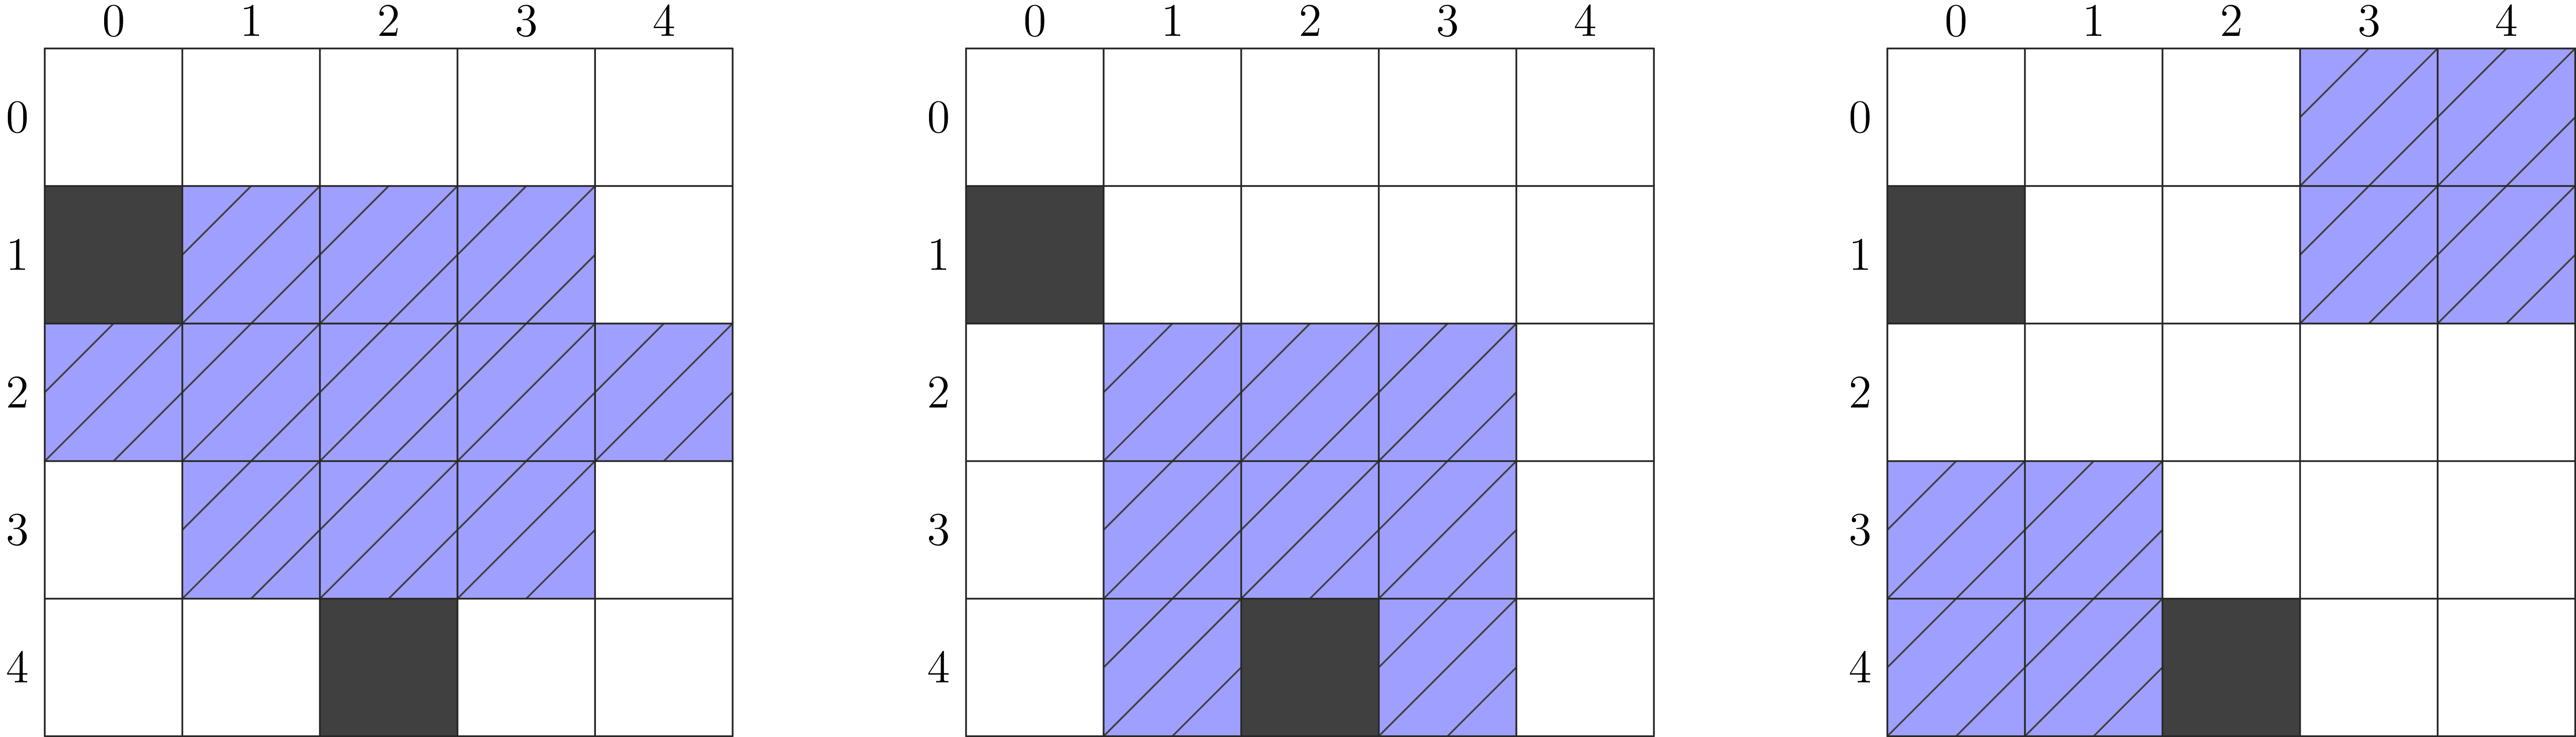
\includegraphics[width=5in]{soccer-example.png}
\caption{Stadiums}
\end{figure}

The stadium on the left is regular. However, the stadium in the middle
is not regular, because at least $3$ straight kicks are needed to move
the ball from cell $(4,1)$ to $(4,3)$. The stadium on the right is
also not regular, because it is impossible to move the ball from cell
$(3,0)$ to $(1,3)$ using straight kicks.

The sports club wants to build a regular stadium that is as big as
possible. Your task is to find the maximum value of $s$ such that
there exists a regular stadium of size $s$ in the forest.

\section*{Implementation Details}

You should implement the following procedure.

\begin{tabular}{| l |}
  \hline
  \verb|int biggest_stadium(int N, int[][] F)| \\
  \hline
\end{tabular}

\begin{itemize}
\item
  $N$: the size of the forest.
\item
  $F$: an array of length $N$ containing arrays of length $N$,
  describing cells in the forest. For each $r$ and $c$ such that
  $0 \le r < N$ and $0 \le c < N$, $F[r][c] = 0$ means that
  cell $(r, c)$ is empty, otherwise $F[r][c] = 1$ means that it
  contains a tree.
\item
  This procedure should return the maximum size of a regular stadium
  that can be built in the forest.
\item
  This procedure is called exactly once for each test case.
\end{itemize}

\section*{Example}

Consider the following call:

\begin{tabular}{| l |}
  \hline
  \verb|biggest_stadium(5, [[0, 0, 0, 0, 0],| \\
  \verb|                    [1, 0, 0, 0, 0],| \\
  \verb|                    [0, 0, 0, 0, 0],| \\
  \verb|                    [0, 0, 0, 0, 0],| \\
  \verb|                    [0, 0, 1, 0, 0]])| \\
  \hline
\end{tabular}

In this example, the forest is displayed on the left and a regular
stadium of size $20$ is displayed on the right of the following
figure:

\begin{figure}[h!]
\centering
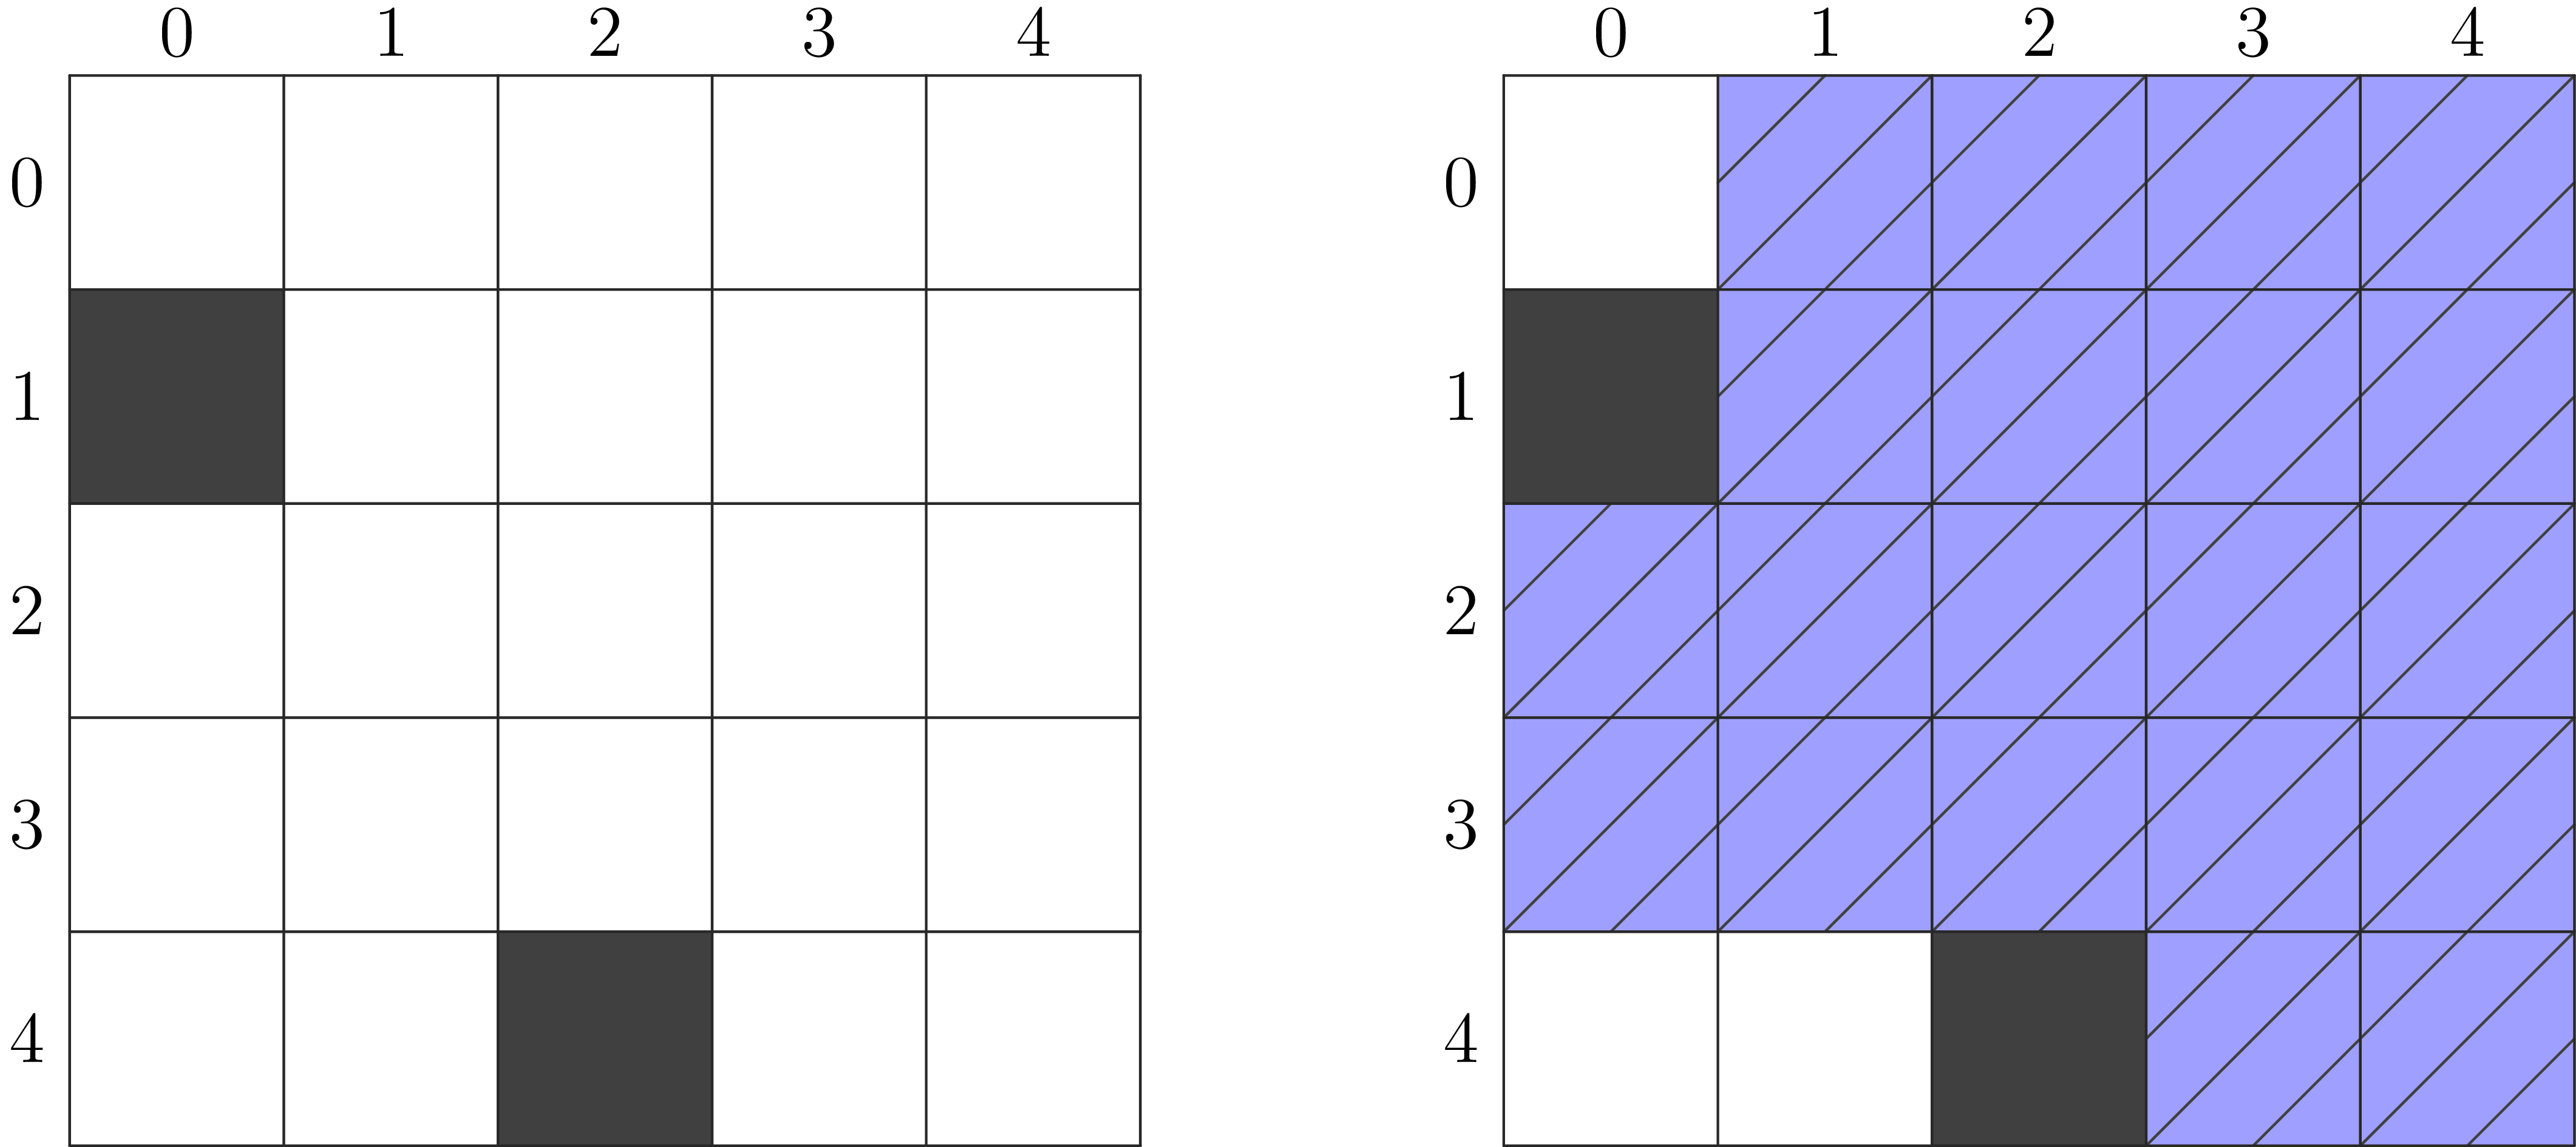
\includegraphics[width=4in]{soccer-regular.png}
\caption{Example}
\end{figure}

Since there is no regular stadium of size $21$ or greater, the
procedure should return $20$.

\section*{Constraints}

\begin{itemize}
\item
  $1 \le N \le 2\,000$
\item
  $0 \le F[i][j] \le 1$ (for each $i$ and $j$ such that
  $0 \le i < N$ and $0 \le j < N$)
\item
  There is at least one empty cell in the forest. In other words,
  $F[i][j] = 0$ for some $0 \le i < N$ and $0 \le j < N$.
\end{itemize}

\section*{Subtasks}

\begin{enumerate}
\def\labelenumi{\arabic{enumi}.}
\item
  (6 points) There is at most one cell containing a tree.
\item
  (8 points) $N \le 3$
\item
  (22 points) $N \le 7$
\item
  (18 points) $N \le 30$
\item
  (16 points) $N \le 500$
\item
  (30 points) No additional constraints.
\end{enumerate}

In each subtask, you can obtain a partial score if your program judges
correctly whether the subset consisting of \emph{all} the empty cells is
a regular stadium.

More precisely, for each testcase in which the subset consisting of all
the empty cells is a regular stadium, your solution:
\begin{itemize}
  \item gets full points
  if it returns the correct answer (which is the size of the subset
  consisting of all the empty cells).
  \item gets 0 points otherwise.
\end{itemize}

For each testcase in which which the subset consisting of all the empty
cells is \emph{not} a regular stadium, your solution:
\begin{itemize}
  \item gets full points if it returns the correct answer.
  \item gets 0 points if it returns the size
  of the subset consisting of all the empty cells.
  \item gets 25\% of the points if it returns any other value.
\end{itemize}

The score for each subtask is the minimum of the points for the test
cases in the subtask.

\section*{Sample Grader}

The sample grader reads the input in the following format:

\begin{itemize}
\item
  line $1$: $N$
\item
  line $2 + i$ ($0 \le i < N$):
  $F[i][0] \; F[i][1] \; \ldots \; F[i][N - 1]$
\end{itemize}

The sample grader prints your answer in the following format:
\begin{itemize}
  \item line $1$: the return value of \texttt{biggest\_stadium}  
\end{itemize}